% This work is licensed under the Creative Commons
% Attribution-NonCommercial-ShareAlike 4.0 International License. To view a copy
% of this license, visit http://creativecommons.org/licenses/by-nc-sa/4.0/ or
% send a letter to Creative Commons, PO Box 1866, Mountain View, CA 94042, USA.

% (c) Eric Kunze, 2019

%%%%%%%%%%%%%%%%%%%%%%%%%%%%%%%%%%%%%%%%%%%%%%%%%%%%%%%%%%%%%%%%%%%%%%%%%%%%
% Template for lecture notes and exercises at TU Dresden.
%%%%%%%%%%%%%%%%%%%%%%%%%%%%%%%%%%%%%%%%%%%%%%%%%%%%%%%%%%%%%%%%%%%%%%%%%%%%

\documentclass[ngerman, a4paper, 12pt]{article}

\usepackage[ngerman]{babel}
\usepackage[top=2.5cm,bottom=2.5cm,left=2.5cm,right=2.5cm]{geometry}
\usepackage{parskip}  	% split paragraphs by vspace instead of intendations
\usepackage[onehalfspacing]{setspace} % increase row-space
\usepackage[title,titletoc]{appendix}

\usepackage[utf8]{inputenc}
\usepackage{chngcntr}
\usepackage{eufrak}

\usepackage{lmodern}
\usepackage[normalem]{ulem} 

\usepackage{fancyhdr} 	% customize header / footer
%\usepackage{tocloft}
%\renewcommand\cftsecafterpnum{\vspace{-pt}}
%\renewcommand{\cfttoctitlefont}{\titlefont\Huge\bfseries}
%\renewcommand{\cftbeforetoctitleskip}{0pt}
%\renewcommand{\cftchapnumwidth}{2em}
%\renewcommand{\cftsecindent}{2em}
%\renewcommand{\cftsecnumwidth}{2em}
%\renewcommand{\cftsubsecindent}{4em}

\usepackage{amsmath,amssymb,amsfonts,mathtools}
\usepackage{blkarray}
\usepackage{latexsym}
\usepackage{marvosym} 	% lightning (contradiction)
\usepackage{stmaryrd} 	% Lightning symbol
\usepackage{bbm} 		% unitary matrix
\usepackage{wasysym}	% add some symbols

\usepackage{systeme}	% easy typesetting systems of equations
\usepackage{witharrows} % arrows from one equation to another

% further support for different equation setting
\usepackage{cancel}
\usepackage{xfrac}		% sfrac -> fractions e.g. 3/4
\usepackage{units}		% units and fractions
\usepackage{diagbox}

\usepackage{../texmf/tex/latex/mathoperatorsMathTUD}

\usepackage[table,dvipsnames]{tudscrcolor}
\usepackage{tabularx} 	% tabularx-environment (explicitly set width of columns)
\usepackage{longtable} 	% Tabellen mit Seitenumbrüchen
\usepackage{multirow}
\usepackage{booktabs}	% improved rules
\usepackage{colortbl}
%\usepackage{subfigure}
\usepackage{flafter,afterpage}
\usepackage[section]{placeins}
\usepackage[margin=8mm,font=small,labelfont=bf,format=plain,justification=centering]{caption}
\usepackage[margin=8mm,font=small,labelfont=bf,format=plain]{subcaption}


\newcommand{\begriff}[1]{\textbf{#1}}
\newcommand{\person}[1]{\textsc{#1}}

%%%%%%%%%%%%%%%%%%%%%%%%%%%%%%%%%%%%%%%%%%%%%%%%%%%%%%%%%%%%%%%%%%%
%                             COUNTER                             %
%%%%%%%%%%%%%%%%%%%%%%%%%%%%%%%%%%%%%%%%%%%%%%%%%%%%%%%%%%%%%%%%%%%
\pretocmd{\chapter}{\setcounter{section}{0}}{}{}
\pretocmd{\chapter}{\setcounter{equation}{0}}{}{}

\usepackage{enumerate}
\usepackage[inline]{enumitem} 		%customize label

\renewcommand{\labelitemi}{\raisebox{2pt}{\scalebox{.4}{$\blacksquare$}}}
\renewcommand{\labelitemii}{$\vartriangleright$}
\renewcommand{\labelitemiii}{--}
% Variantionen des Dreiecks als Aufzählungszeichen $\blacktriangleright$ / $\vartriangleright$ / $\triangleright$

\renewcommand{\labelenumi}{(\arabic{enumi})}
\renewcommand{\labelenumii}{\alph{enumii}.}
\renewcommand{\labelenumiii}{\roman{enumiii}.}

%%%%%%%%%%%%%%%%%%%%%%%%%%%%%%%%%%%%%%%%%%%%%%%%%%%%%%%%%%%%%%%%%%%
\usepackage{titlesec}   % change title headings look
\usepackage{chngcntr}   % modify counters
\usepackage{relsize}    % relative font size (smaller[i], larger[i], ...)


%%%%%%%%%%%%%%%%%%%%%%%%%%%%%%%%%%%%%%%%%%%%%%%%%%%%%%%%%%%%%%%%%%%
% headings
%%%%%%%%%%%%%%%%%%%%%%%%%%%%%%%%%%%%%%%%%%%%%%%%%%%%%%%%%%%%%%%%%%%
\newcommand{\titlefont}{\osfamily}
\newcommand{\chaptersize}{\huge}
\newcommand{\sectionsize}{\LARGE}

\renewcommand{\thepart}{\Alph{part}}

% \titleformat{<command>}[<shape>]{<format>}{<label>}{<sep>}{<before-code>}[<after-code>]
% \titlespacing*{<command>}{<left>}{<before-sep>}{<after-sep>}[<right-sep>]

%%%%%%%%% section
%\titlelabel{\thetitle \quad} % no "." behind section/sub... (3 instead of 3.)
\titleformat{\section}[hang]{\bfseries\LARGE}{\thesection}{8pt}{}%
%\titleformat*{\section}{\bfseries\titlefont\sectionsize}
%\titleformat*{\subsection}{\bfseries\titlefont\sectionsize\smaller}

%%%%%%%%%%%%%%%%%%%%%%%%%%%%%%%%%%%%%%%%%%%%%%%%%%%%%%%%%%%%%%%%%%%

\usepackage{listings}

%%%%%%%%%%%%%%%%%%%%%%%%%%%%%%%%%%%%%%%%%%%%%%%%%%%%%%%%%%%%%%%%%%%
%                           REFERENCES                            %
%%%%%%%%%%%%%%%%%%%%%%%%%%%%%%%%%%%%%%%%%%%%%%%%%%%%%%%%%%%%%%%%%%%

\usepackage{titlesec}   % change title headings look
\usepackage{relsize}    % relative font size (smaller[i], larger[i], ...)

\usepackage{titling}
%\pretitle{\begin{center}\Huge\bfseries\sffamily}
%\posttitle{\par}
%\preauthor{\par \normalfont \large \scshape}
%\postauthor{\par}
%\postdate{\end{center}

\DeclareMathSymbol{*}{\mathbin}{symbols}{"01}

\counterwithin{equation}{section}
\newcounter{themcount}
\counterwithin{themcount}{section}
%\usepackage{amsmath,amssymb,amsfonts,mathtools}
\usepackage[amsmath,thmmarks,framed]{ntheorem}

\newcommand{\skiparound}{10pt}
\theorempreskip{\skiparound}
\theorempostskip{\skiparound}

\theoremstyle{plain}
\theoremseparator{.}
\theorembodyfont{}
\newtheorem{definition}[themcount]{Definition}
\newtheorem{bemerkung}[themcount]{Bemerkung}

\newtheorem{beispiel}[themcount]{Beispiel}

\theorembodyfont{\itshape}
\newtheorem{satz}[themcount]{Satz}
\newtheorem{lemma}[themcount]{Lemma}


\theoremstyle{break}
\theorembodyfont{\upshape}
\newtheorem{algorithmus}[themcount]{Algorithmus}

\makeatletter
\newtheoremstyle{proofstyle}{\item[\hskip\labelsep {\theorem@headerfont ##1}\theorem@separator]}{\item[\hskip\labelsep {\theorem@headerfont ##1}\ (##3)\theorem@separator]}
\makeatother

\theoremstyle{proofstyle}
\theoremheaderfont{\normalsize\slshape}
\theorembodyfont{}
\theoremseparator{.}
\theorempreskip{5pt}
\theorempostskip{5pt}
\theoremsymbol{$\square$}
\newtheorem{proof}{Beweis}


\newcommand{\ianfang}[1][]{%
	\ifthenelse{\isempty{#1}}{%
		% no parameter
		\item[\textbf{(IA)}]%
	}{%
		%parameter exists
		\item[\textbf{(IA)}] {#1 :} %\hfill \\%
	}%
}

\newcommand{\ivoraussetzung}{\item[\bfseries (IV)]}

\newcommand{\ischritt}[1][]{%
	\ifthenelse{\isempty{#1}}{%
		% no parameter
		\item[\textbf{(IS)}]
	}{%
		% parameter exists
		\item[\textbf{(IS)}] {#1 :} %\\
	}%
}

% two optional arg's:
% #1 = induced variable 
% #2 = vert. space before (IA): parskip (default) or nopreskip
\NewDocumentEnvironment{induction}{O{} O{}}{%
	\ifthenelse{ \isempty{#1} }{}{%
		Vollständige Induktion nach #1:
	}%---
	\ifthenelse{ \equal{#2}{nopreskip} }{%
		\begin{description}[topsep=-\parskip]
		}{%
			\begin{description}
			}%
		}{%
		\end{description}%
	}
	
\DeclareMathOperator{\GE}{GE}
\DeclareMathOperator{\VF}{VF}

\usepackage[
type={CC},
modifier={by-nc-sa},
version={4.0},
]{doclicense}

\usepackage[unicode,bookmarks=true]{hyperref}
\hypersetup{
	% pdfborder={0 0 0}			% no boxed around links
	pdfborderstyle={/S/U/W 1},	% underlining insteas of boxes
	linkbordercolor=cdblue,
	urlbordercolor=cdblue
	%	colorlinks,
	%	citecolor=black,
	%	filecolor=cddarkblue!80,
	%	linkcolor=black,
	%	urlcolor=cddarkblue!80
}

\usepackage{cleveref}
\crefname{satz}{Satz}{Sätze}
\crefname{lemma}{Lemma}{Lemmata}
\crefname{definition}{Definition}{Definitionen}
\crefname{bemerkung}{Bemerkung}{Bemerkungen}
\crefname{beispiel}{Beispiel}{Beispiele}
\crefname{algorithmus}{Algorithmus}{Algorithmen}

\usepackage{bookmark}		% pdf-bookmarks


\begin{document}
	\title{\bfseries \sffamily \huge Knotenfärbung \& Vier-Farben-Satz}
	\author{\scshape Eric Kunze}
	\date{29.~Januar~2020}
	\maketitle
	{ \footnotesize \doclicenseThis }
	
	\singlespacing
	\tableofcontents
	\onehalfspacing
	
	\vspace{\parskip}
	
	Der Vortrag stützt sich zu großen Teilen auf die Ausführungen in \cite{buesing} und wurde um einige zusätzliche Resultate ergänzt.
	
\section{Knotenfärbung}
	
	\begin{definition}
		Eine \begriff{(Knoten)-Färbung} eines Graphen $G = (V,E)$ ist eine Abbildung $\abb{c}{V}{S}$ mit einer beliebigen Menge $S$, sodass
		\begin{equation}
			\label{eq: faerbung}
			c(u) \neq c(v) \text{ für alle } u,v \in V \mit (u,v) \in E
		\end{equation}
		Die Elemente von $S$ heißen \begriff{Farben}.
	\end{definition}

	\begin{definition}
		Ein Graph ist \begriff{$k$-färbbar}, falls es eine Färbung $\abb{c}{V}{\menge{1, \dots, k}}$ gibt. Das kleinste $k$, für das
		$G$ noch $k$-färbbar ist, ist die \begriff{chromatische Zahl} $\chi(G)$ von $G$.
	\end{definition}

	Für $G = (V,E)$ gilt 
	\begin{equation}
		1 \le \chi(G) \le \card{V}
		\label{eq: chi-kleiner-n}
	\end{equation}
	Nun stellt sich die Frage, wie man eine gültige Färbung eines Graphen erhält. Dies beantwortet der folgende Algorithmus.

	\begin{algorithmus}[Färbungsalgorithmus]
		\label{alg: faerbung}
		\begin{itemize}[nolistsep]
			\item Input: Graph $G = (V,E)$ mit $\card{V} = n$ 
			\item Output: Färbung $\abb{c}{V}{\menge{1, 2, \dots }}$
		\end{itemize}
		\begin{enumerate}[label=Schritt \arabic*:, leftmargin=*, nolistsep]
			\item Nummeriere die Knoten mit $v_1, \dots, v_n$
			\item Färbe den Knoten $v_1$ mit der Farbe $1$
			\item Betrachte der Reihenfolge nach alle Knoten und färbe diese mit der kleinst"-möglichen Farbe
		\end{enumerate}
	\end{algorithmus}

	Diese Abschätzung in \cref{eq: chi-kleiner-n} lässt sich unter Nutzung des Maximalgrades eines Graphen noch verschärfen. Wir bezeichnen mit $\Delta(G)$ den Maximalgrad von $G$, also $\Delta(G) \defeq \max\menge{d(v) : v \in V}$.
	
	\begin{satz}
		Sei $G = (V,E)$ ein Graph. Dann gilt
		\begin{equation}
			1 \le \chi(G) \le \Delta(G) + 1
			\label{eq: chi-kleiner-delta+1}
		\end{equation}
	\end{satz}
	\begin{proof}
		Wir betrachten einen Knoten $v \in V$ mit $d(v) = \Delta(v)$. \cref{alg: faerbung} färbt die $\Delta(v)$ vielen Nachbarknoten von $v$ mit einer von $v$ verschiedenen Farbe. Demnach brauchen wir also für den \enquote{schlechtesten} Knoten $\Delta(G) + 1$ viele verschiedene Farben.
	\end{proof}
	
	Die Abschätzung in \cref{eq: chi-kleiner-delta+1} in tatsächlich scharf, d.h. es gibt Graphen $G$, für die $\chi(G) = \Delta(G) + 1$ gilt:
	\begin{center}
		\begin{tabular}{ccc}
			Kreise ungerader Länge && vollständige Graphen \\
			z.B. $G = K_3$ & & z.B. $G = K_4$ \\
			\includegraphics[scale=1]{k3.pdf} 
			& \hspace{3em} &
			\includegraphics[scale=1]{k4.pdf}
		\end{tabular}
	\end{center}
	
	Jedoch sind diese Klassen von Graphen auch schon die einzigen, die \cref{eq: chi-kleiner-delta+1} mit Gleichheit erfüllen.
	Somit kommt man in allen anderen Fällen in \cref{alg: faerbung} auch mit $\Delta(G)$ vielen Farben aus.
	Die Idee dahinter ist eine clevere Anordnung der Knoten vor der Farbzuweisung. Kritisch sind nämlich nur die Fälle, in denen ein Knoten Maximalgrad hat, denn dann benötigt man bereits $\Delta(G)$ viele Farben für die Nachbarn und im Zweifelsfall eine weitere für den Knoten selbst. In vielen Fällen bleibt aber vor dem letzten Knoten eine Farbe übrig, sodass \cref{alg: faerbung} keine zusätzliche beanspruchen muss.
 	
	\begin{satz}[Brooks]\label{satz: brooks}
		Sei $G$ ein zusammenhängender Graph mit mehr als zwei Knoten.
		\begin{enumerate}[label=(\roman*), nolistsep, topsep=-\parskip]
			\item Ist $G$ vollständig oder ein Kreis ungerader Länge, dann gilt $\chi(G) = \Delta(G) + 1$.
			\item Andernfalls gilt $\chi(G) \le \Delta(G)$.
		\end{enumerate}
	\end{satz}
	\begin{proof}
		Die Aussage (i) ist mit den obigen Beispielen klar. Aussage (ii) zeigen wir in mehreren Schritten und folgen dabei \cite{Cranston2014}.
		\begin{enumerate}[label=Fall \arabic* ---, leftmargin=*, itemindent=*]
			\item Wir beschränken uns zunächst auf den Fall, dass $G$ nicht regulär ist, d.h. nicht alle Knoten Maximalgrad $\Delta \defeq \Delta(G)$ haben. 
			Für $\Delta(G) \le 2$ ist $G$ ein Weg oder Kreis und die Aussage ist damit klar. Sei daher von nun an $\Delta(G) \ge 3$.
			Vollständige Induktion nach $\card{V}$ --- Im Induktionsanfang betrachten wir $\card{V} = 3$, d.h. einen Graphen mit genau drei Knoten. Aufgrund der Annahme $\Delta(G) \ge 3$ ist hier nichts zu zeigen. 
			
			In der Induktionsvoraussetzung nehmen wir an, dass $\chi(H) \le \Delta(H)$ für alle Graphen $H$ mit $\card{H} < \card{G}$. 
			
			Im Induktionsschritt wählen wir einen Knoten $v \in V$ mit $d(v) < \Delta(G)$. Dieser existiert, weil gemäß unserer Annahme nicht alle Knoten Maximalgrad haben. 
			Betrachten wir den Graphen $H \defeq G - v$. 
			Dieser besitzt weniger Knoten als $G$, also hat auch kein Knoten in $H$ mehr Nachbarn als in $G$. Diese Einsicht liefert $\Delta(H) \le \Delta(G)$ und mit der Induktionsvoraussetzung $\chi(H) \le \Delta(H)$ existiert also insbesondere auch eine $\Delta$-Färbung von $H$. 
			Es verbleibt nun noch der Knoten $v$ zu färben. Da $v$ nur $d(v) < \Delta$ viele Nachbarn hat, bleibt mindestens eine der $\Delta$ vielen Farben für $v$ übrig und wir erhalten damit eine $\Delta$-Färbung von $G$.
		
			\item Ist $G$ regulär, d.h. alle Knoten besitzen Maximalgrad $\Delta$, dann existiert ein Knoten $v$ wie oben nicht mehr. Ist $v$ aber zumindest ein Artikulationspunkt, d.h. $H \defeq G - v$ zerfällt in Komponenten, dann lässt sich das obige Verfahren noch retten. Sei dazu $H'$ eine Komponente von $H$. Diese besitzt gemäß Induktionsvoraussetzung wie oben eine $\Delta$-Färbung. Diese kann ebenso wie oben zu einer $\Delta$-Färbung von $H' + v$ fortgesetzt werden, weil $v$ in $H' + v$ nicht Maximalgrad hat (es fehlen die anderen Zusammenhangskomponenten, die \enquote{an $v$ hängen}). Setzt man dieses Verfahren für alle Komponenten von $H$ ein, erhält $v$ unter Umständen jedes Mal eine andere Farbe. Dies behebt man, indem die Farben so zyklisch vertauscht (permutiert), dass $v$ immer die gleiche Farbe bekommt. Dies stellt am Ende eine $\Delta$-Färbung von $G$ dar.
		
			\item Der verbleibende Fall beschäftigt sich nun mit $\Delta$-regulären Graphen, die zweifach zusammenhängend sind, also weder einen Artikulationspunkt noch einen Knoten $v$ mit $d(v) < \Delta(v)$ besitzen. In diesem Fall kann man zeigen, dass es einen induzierten Pfad\footnote{Ein induzierter Pfad ist ein Pfad, der gleichzeitig ein induzierter Teilgraph von $G$ ist. Er ist also eine Folge von Knoten, sodass zwei im Pfad benachbarte Knoten mit einer Kante in $G$ verbunden sind und zwei nicht-benachbarte Knoten im Pfad keine Kante in $G$ besitzen. Ein induzierter Pfad wird auch Schlange genannt.} $uvw$ in $G$ gibt, sodass $H \defeq G - \menge{u, w}$ zusammenhängend ist. Färbt man nun die Knoten $u$ und $w$ gleich und verfährt mit $H$ wie im ersten Fall, dann bleibt erneut eine der $\Delta$ Farben für $v$ übrig, da mit $u$ und $w$ zwei Nachbarn gleiche Farben haben.
		\end{enumerate}
	\end{proof}

	\begin{figure}[hb]
		\centering
		\begin{tabular}{ccc}
			\includegraphics[page=2]{brooks.pdf}
			& \hspace{3em} &
			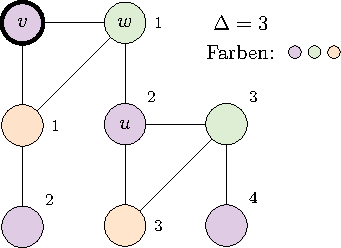
\includegraphics[page=1]{brooks.pdf}
		\end{tabular}
		\caption{Variante von \cref{alg: faerbung} zum Beweis von \cref{satz: brooks}. Die Reihenfolge der Färbung ist durch die Zahlen dargestellt. Der Knoten $u$ hat Maximalgrad $d(u) = 3 = \Delta$. Da es auf dem Weg von $v$ zu $u$ aber den ungefärbten Nachbarn $w$ von $u$ gibt, bleibt mindestens eine Farbe übrig, diese erhält $u$.}
	\end{figure}

	Mithilfe von \cref{alg: faerbung} sieht man auch leicht das folgende Resultat.
	
	\begin{satz}[\cite{bodirsky}]
		Ein endlicher Graph $G$ ist genau dann zweifärbbar, wenn er keine ungeraden Kreise enthält.
	\end{satz}

	Nun haben wir die chromatische Zahl $\chi(G)$ gut bezügliche der Anzahl an Knoten abgeschätzt. Im Folgenden wollen wir noch eine Abschätzung in Hinblick auf die Kantenzahl erzielen.
	
	\begin{satz}[\cite{diestel}]
		Sei $G = (V,E)$ ein Graph mit $\card{E} = m$. Dann gilt
		\begin{equation}
			1 \le \chi(G) \le \frac{1}{2} + \sqrt{2m + \frac{1}{4}}
			\label{eq: chi-kanten}
		\end{equation}
	\end{satz}
	\begin{proof}
		Wir betrachten eine $k = \chi(G)$-Färbung $c$ von $G$ und entstehenden Farbklassen $c^{-1}(i)$. Betrachten wir zwei solche Farbklassen $c^{-1}(i)$, dann muss zwischen diesen beiden Klassen mindestens eine Kante existieren, da diese sonst gleich eingefärbt werden könnten und folglich zur gleichen Farbklasse gehörten. Jede der $k$ Klassen hat also mindestens $k-1$ Kanten zu den benachbarten Klassen. Nun haben wir allerdings die Kanten doppelt gezählt, d.h. es gilt
		\begin{equation*}
			m \ge \frac{1}{2} k (k-1) \follows k \le \frac{1}{2} + \sqrt{2m + \frac{1}{4}}
		\end{equation*}
	\end{proof}

	Wir können also mittlerweile einen Graphen $G$ färben und die dazu benötigte Anzahl an Farben auch eingrenzen. Doch wie bestimmt man nun die chromatische Zahl $\chi(G)$ exakt? Dafür können wir \cref{alg: faerbung} wie folgt nutzen.
	\begin{enumerate}[nolistsep, topsep=-\parskip]
		\item Angenommen wir kennen für einen Graphen $G$ eine $\chi(G)$-Färbung.
		\item Sortiere nun die Knoten nach ihren Farben.
		\item Starte den Färbungsalgorithmus mit dieser neuen Sortierung
	\end{enumerate}
	Man sieht leicht, dass der Algorithmus wieder eine $\chi(G)$-Färbung liefert.
	
	Somit liegt die Idee nahe, \enquote{einfach} alle möglichen Anordnungen zu testen um am Ende die minimale Anzahl an Farben als chromatische Zahl zu setzen. Jedoch sind dabei im Allgemeinen $\card{V}!$ viele Fälle zu testen, was dieses Verfahren ineffizient macht.
	
	Aus komplexitätstheoretischer Sicht ist die Bestimmung der chromatischen Zahl sogar ein NP-vollständiges Problem, d.h. es existiert vermutlich auch kein Algorithmus, der dieses Problem effizient lösen kann.
	
\pagebreak

	\section{Vier-Farben-Problem}
	
	Wir betrachten eine Landkarte und wollen diese Einfärben unter Beachtung der Bedingung, dass aneinander grenzende Länder unterschiedlich gefärbt werden sollen. Wie viele Farben benötigen wir dafür?
	
	Um das Problem zu lösen benötigen wir zuerst eine mathematische Modellierung, welche wir in dualen Graphen finden.
	
	\begin{definition}
		Sei $G = (V,E)$ ein planarer Graph. Der \begriff{duale Graph} $G^\ast = (V^\ast, E^\ast)$ zu einer planaren Darstellung von $G$ hat in jeder Fläche von $G$ genau einen Knoten. Außerdem gibt es für jede Kante $e \in E$ genau eine Kante $e^\ast \in E^\ast$, die die an $e$ anliegenden Flächen verbindet.
	\end{definition}

	\begin{bemerkung}
		Die Darstellung des dualen Graphen $G^\ast$ hängt von der planaren Darstellung des Graphen $G$ ab und ist somit im Allgmeinen nicht eindeutig. Durch in Flächen hineinragende Kanten von $G$ können Schlingen in $G^\ast$ entstehen. 
	\end{bemerkung}

	\begin{bemerkung}
		Planarität überträgt sich auf den Dualgraphen. Betrachte dazu das folgende Vorgehen:
		\begin{enumerate}[nolistsep, topsep=-\parskip]
			\item zeichne alle Knoten des Dualgraphen $G^\ast$ ein
			\item halbiere alle Kanten in $G$
			\item verbinde nun die Knoten mit den Halbierungspunkten durch \enquote{Kurven}
		\end{enumerate}
	\end{bemerkung}

	Nun haben wir unsere Landkarte in ein mathematisches Modell übertragen.  Der folgende Satz erklärt uns, dass wir den daraus entstandenen (planaren) Graphen mit vier Farben einfärben können.

	\begin{satz}[Vier-Farben-Satz]
		Jeder planare Graph lässt sich mit vier Farben färben.
	\end{satz}

	Der Beweis des Vier-Farben-Satzes ist bis heute nur mit einem Computer erbracht worden. Daher steht eine \enquote{endgültige}, für den Menschen verständliche Lösung des Problems noch aus.
	
	Wir wollen dennoch eine zumindest abgeschwächte Variante zeigen, nämlich den Fünf-Farben-Satz. Dafür erinnern wir uns zuerst an ein bekanntes Resultat, welches wir für den nachfolgenden Satz verwenden wollen.
	
	\begin{lemma}
		\label{lemma: planar5Knoten}
		Jeder planare Graph hat mindestens einen Knoten mit höchstens fünf Nachbarn.
	\end{lemma}

	
	\begin{satz}[Fünf-Farben-Satz]
		Jeder planare Graph ist mit fünf Farben färbbar.
	\end{satz}
	\begin{proof} vollständige Induktion nach $n = \card{V}$:
		\begin{description}
		\ianfang Für $n \le 5$ ist die Aussage klar.
		\ivoraussetzung Jeder planare Graph mit weniger als $n$ Knoten ist fünffärbbar.
		\ischritt Sei $G = (V,E)$ ein planarer Graph in planarer Darstellung. Nach \cref{lemma: planar5Knoten} existiert ein Knoten $v \in V$ mit höchstens fünf Nachbarn (d.h. $d(v) \le 5$)
		\begin{enumerate}[label=Fall \arabic*:]
			\item $d(v) \le 4$ --- Lösche $v$ aus $G$ und betrachte $G' \defeq G - v$. Dieser hat nur noch $n-1$ Knoten und ist nach Induktionsvoraussetzung entsprechend mit fünf Farben färbbar. Insbesondere benötigen wir für die vier Nachbarn von $v$ auch maximal vier Farben. Fügen wir also $v$ wieder hinzu  und färben diesen Knoten mit der übrigen Farbe, so erhalten wir eine gültige $5$-Färbung von $G$. 
			\item $d(v) = 5$ --- Betrachten wir wieder $G' \defeq G - v$ und finde eine zulässige $5$-Färbung nach Induktionsvoraussetzung. Werden für die fünf Nachbarn nur vier Farben benötigt, so können wir wie in Fall 1 verfahren und $v$ mit der übrigen Farbe färben. Nehmen wir also an, dass für alle fünf Nachbarn mit paarweise verschiedenen Farben gefärbt worden sind -- nummeriere die Nachbarn mit $v_1, \dots, v_5$ im Uhrzeigersinn, wobei der Index gleichzeitig auf die Farbe repräsentieren soll, die der entsprechende Knoten nach Induktionsvoraussetzung bekommen hat. Das Ziel ist nun durch Umfärben der Knoten $v_1, \dots, v_5$ eine Farbe einzusparen. Betrachte dazu $H_{1,3}$, den Teilgraphen von $G'$, der von den Knoten $v_1$ und $v_3$ induziert wird.
			\begin{enumerate}[label=\alph*),topsep=-\parskip]
				\item Wir nehmen an, dass es in $H_{1,3}$ keine Weg von $v_1$ nach $v_3$ gibt. Dann können wir in der Zusammenhangskomponente, die $v_1$ enthält die Knoten umfärben durch
				\begin{equation*}
					\text{Farbe } 1 \leftrightarrow \text{ Farbe } 3
				\end{equation*}
				Damit ist $v_1$ nun mit Farbe $3$ gefärbt und wir können $v$ nach Hinzufügen die Farbe $1$ zuweisen.
				\item Angenommen die Knoten $v_1$ und $v_3$ sind in $H_{1,3}$ durch einen Weg verbunden. Da wir durch Umfärben in $H_{1,3}$ nichts erreichen würden, betrachten wir $H_{2,4}$. Zwischen $v_2$ und $v_4$ kann nun kein Weg in $H_{2,4}$ existieren, da $G$ planar dargestellt war; wie oben bringt also Umfärben
				\begin{equation*}
					\text{Farbe } 2 \leftrightarrow \text{ Farbe } 4
				\end{equation*}
				in der Zusammenhangskomponente von $v_2$ eine neue Färbungsmöglichkeit für $v$ mit Farbe $2$.
			\end{enumerate}
		\end{enumerate}
		Somit haben wir in jedem Fall eine gültige $5$-Färbung für $G$ gefunden.
		\end{description}
	\end{proof}

	\section{Färbung und SAT}
	
	Wir wollen im Folgenden noch kurz den komplexitätstheoretischen Zusammenhang zwischen der Graphenfärbung und dem Erfüllbarkeitsproblem der Aussagenlogik (SAT) anreißen. Letzteres besteht darin, für eine gegebene aussagenlogische Formel $F$ eine Variablenbelegung zu finden, die die Formel auf wahr abbildet.
	Wir nutzen dazu die Konstruktion in \cite{mehlhorn}.

	\begin{satz}[Färbung $\preccurlyeq$ SAT]
		\label{satz: faerbung-sat}
		Falls SAT effizient lösbar ist, dann ist auch Graphen"-färbung effizient lösbar --- Gegeben sei ein Graph $G$. Konstruiere nun eine Formel $F$ mit
		\begin{itemize}[nolistsep, topsep=-\parskip]
			\item $G$ ist genau dann ($k$-) färbbar, wenn $F$ erfüllbar ist.
			\item Die Konstruktion von $F$ aus $G$ ist in Polynomialzeit durchführbar.
		\end{itemize}
	\end{satz}

	\begin{beispiel}[$3$-Färbbarkeit]
		Sei $G = (V,E)$ ein $3$-färbbarer Graph mit Farben $S = \menge{a,b,c}$. Wir wollen nun daraus eine Formel wie in \cref{satz: faerbung-sat} finden und definieren (aussagenlogische) Variablen $x_a = \top$ genau dann, wenn der Knoten $v$ mit Farbe $a$ gefärbt worden ist.
		Nun müssen wir zwei Eigenschaften modellieren:
		\begin{itemize}
			\item Jeder Knoten hat eine eindeutige Farbe --- Dazu definieren wir uns ein Prädikat $\GE$, das genau dann auf wahr abgebildet wird, wenn genau eines der Argumente wahr ist:
			\begin{equation*}
				\GE (x,y,z) = (x \lor y \lor z) \land \lnot ((x \land y) \lor (x \land z) \lor (y \land z))
			\end{equation*}
			Damit lässt sich die Eigenschaft genau eine Farbe zu tragen mit
			\begin{equation*}
				\bigwedge_{v \in V} \GE(v_a, v_b, v_c)
			\end{equation*}
			in die Sprache der Aussagenlogik übersetzen.
			\item Für alle $(u,v) \in E$ haben $u$ und $v$ verschiedene Farben (vgl. \eqref{eq: faerbung}) --- Definieren wir ein Prädikat $\VF(u,v)$, das dann wahr ergibt, wenn $u$ und $v$ verschiedene Farben tragen:
			\begin{equation*}
				\VF(u,v) = \lnot ((u_a \land v_a) \lor (u_b \land v_b) \lor (u_c \land v_c))
			\end{equation*}
			Die Eigenschaft \eqref{eq: faerbung} lässt sich also formulieren als
			\begin{equation*}
				\bigwedge_{(u,v) \in E} \VF(u,v)
			\end{equation*}
		\end{itemize}
		Schlussendlich ist die \enquote{zu $G$ äquivalente} Formel gegeben durch
		\begin{equation*}
			F = \bigwedge_{v \in V} \GE(v_a, v_b, v_c) \land \bigwedge_{(u,v) \in E} \VF(u,v)
		\end{equation*}
	\end{beispiel}
	
	\nocite{*}	
	\bibliographystyle{alphadin} %alternativ:  abbrvdin alphadin natdin plaindin unsrtdin
	\bibliography{literatur}
 
\end{document}

